\appendix
\backupbegin

\section{Gapped consecutive matching}

\begin{frame}
  \centering
  {\Large Gapped Consecutive Matching}

  \bigskip
  \begin{minipage}{0.55\textwidth}  
    \begin{enumerate}
      \item Grammar Compressed Indexing (CPM'23)
      \item Grammar Compressed Pattern Matching
    \end{enumerate}
  \end{minipage}\\
  \bigskip
  
  
\includegraphics{pictures/mindmap/gapped.png}

  \bigskip
  Paweł Gawrychowski, Tatiana Starikovskaya, Teresa Anna Steiner
\end{frame}


%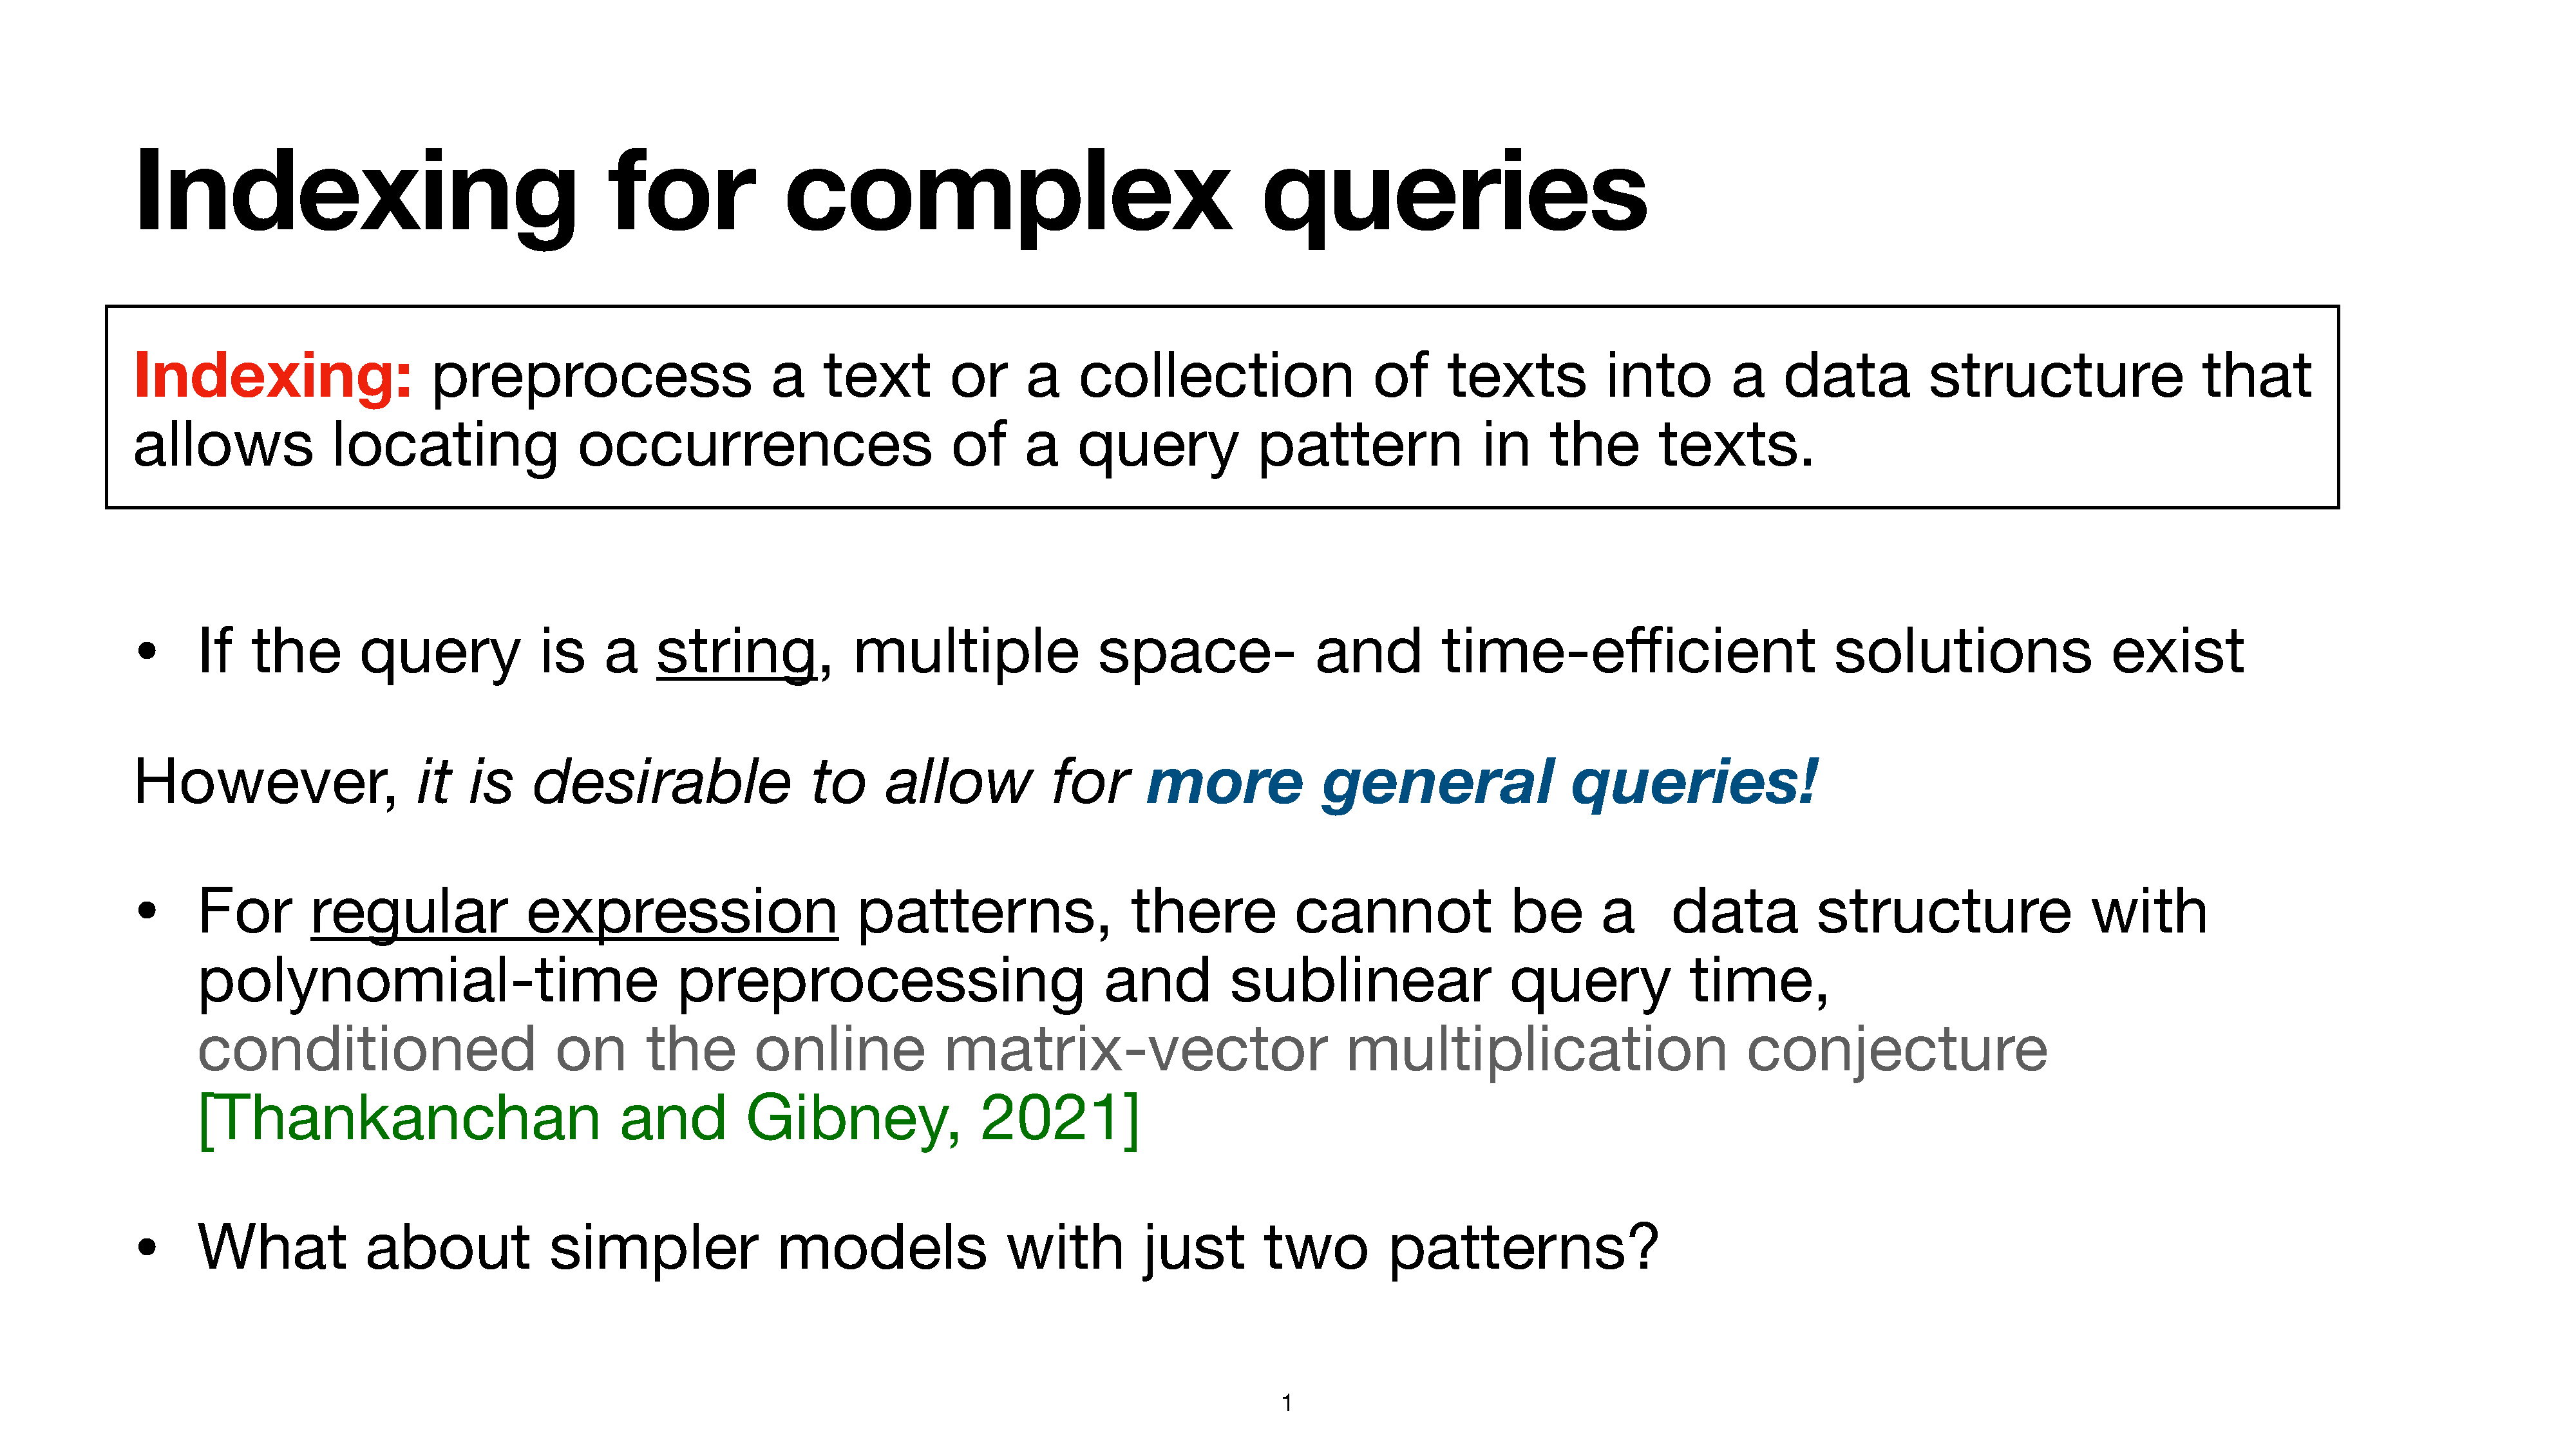
\includepdf[pages={-}]{pdf/2_index_gapped.pdf}



\newcommand{\kLCS}{\textsf{LCS with $k$ Mismatches}}
\newcommand{\kApproxLCS}{\textsf{LCS with Approximately $k$ Mismatches}}
\newcommand{\acs}{\mathrm{ACS}}
\newcommand{\lcpk}{\mathrm{LCP}_{k}}
\newcommand{\lcpe}{\mathrm{LCP}_{(1+\eps)k}}
\newcommand{\Projections}{\Pi}
\newcommand{\Hashes}{\mathcal{H}}
\newcommand{\Collisions}{C}
\newcommand{\HD}{d_H}
\newcommand{\sk}{\mathrm{sk}}
\newcommand{\norm}[1]{\ensuremath{\lVert#1\rVert}}
\newcommand{\Ham}{\mathrm{Ham}}


\subsection{LCS(ubstring) with Approximately k Mismatches}
\begin{frame}
  \centering
  \beamermathcolor{black}
  {\Large The Longest Common Substring with Approximately $k$ Mismatches}
  
  \medskip
  {\large CPM'20}
  \bigskip

  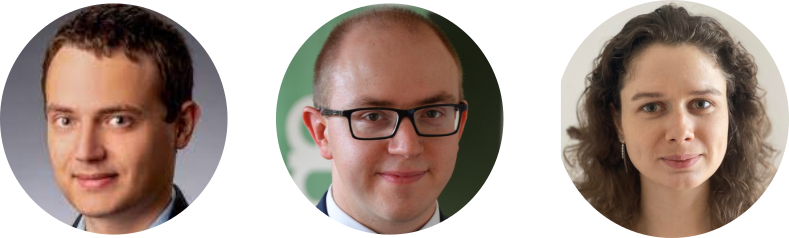
\includegraphics{pictures/mindmap/lcsk.png}

  \bigskip
  Tomasz Kociumaka, Jakub Radoszewski, Tatiana Starikovskaya
\end{frame}


\frame{
\frametitle{The Longest Common Substring with Approximately $k$ mismatches}
\begin{block}{$LCS_{\tilde{k}}$}
\textbf{Input}: Two strings $X, Y$ of length $n$, an integer $k$.\\
\textbf{Output}: A substring of $X$ of length at least $LCS_k$ that occurs in $Y$ with at most $(1+\eps) \cdot k$ mismatches.
\end{block}

\pause

\begin{block}{[Kociumaka, Radosweski, Starikovskaya'19]}
  $LCS_{\tilde{k}}$ can be solved for $\eps < 2$, in $\Oh(n^{1+1/(1+\eps)}\log^2 n)$ time and $\Oh(n^{1+1/(1+\eps)})$ space.
\end{block}

}

\frame{
\frametitle{Our contributions}
\begin{myalertblock}{Upper bounds}
 Let $\eps > 0$ be an arbitrary constant. The \kApproxLCS  problem can be solved correctly with high probability: 
\begin{enumerate}[1)]
\item in $\Oh(n^{1+ 1/(1+2\eps) + o(1)} \log^2 n)$ time and $\Oh(n^{1+ 1/(1+2\eps) + o(1)})$ space assuming a constant-size alphabet;
\item and $\Oh(n^{1+1/(1+\eps)} \log^3 n)$ time and $\Oh(n)$ space for alphabets of arbitrary size. 
\end{enumerate}
\end{myalertblock}

\begin{myalertblock}{Lower Bound}
Assuming SETH, for every constant $\delta > 0$, there exists a constant $\eps = \eps(\delta)$ such that given $X$ and $Y$ of size $n$ computing the \kApproxLCS requires $\Omega(n^{2-\delta})$ time. 
\end{myalertblock}
}


\frame{
\frametitle{The Longest Common Substring problem}

\begin{block}{LCS}
\textbf{Input}: Two strings $X, Y$ of length $n$.\\
\textbf{Output}: The longest substring that occurs both in $X$ and $Y$.
\end{block}

Issue: It is not robust.
\pause
\begin{center}
$X=a^{2m+1}$ and $Y= a^{2m}b$ $\Rightarrow$ $LCS(X,Y)=2m$\\
\pause
$X=a^{m}ba^m$ and $Y= a^{2m}b$ $\Rightarrow$ $LCS(X,Y)=m$
\end{center}
\pause
Only one character changed, and the LCS has been divided by 2.
}


\frame{
\frametitle{The Longest Common Substring with $k$ mismatches}
\begin{block}{\kLCS}
\textbf{Input}: Two strings $X, Y$ of length $n$, an integer $k$.\\
\textbf{Output}: A substring of $X$ that occurs in $Y$ with at most $k$ mismatches.
\end{block}
\pause
However...
\begin{block}{[Kociumaka, Radoszweski, Starikovskaya'19]}
 There is a $k = \Theta (\log(n))$ such that $LCS_k$ can't be computed in strongly subquadratic time, unless SETH is false.
 \end{block}

}


\frame{
\frametitle{Twenty question game with a liar}

\begin{center}
\hspace{0.1\textwidth}
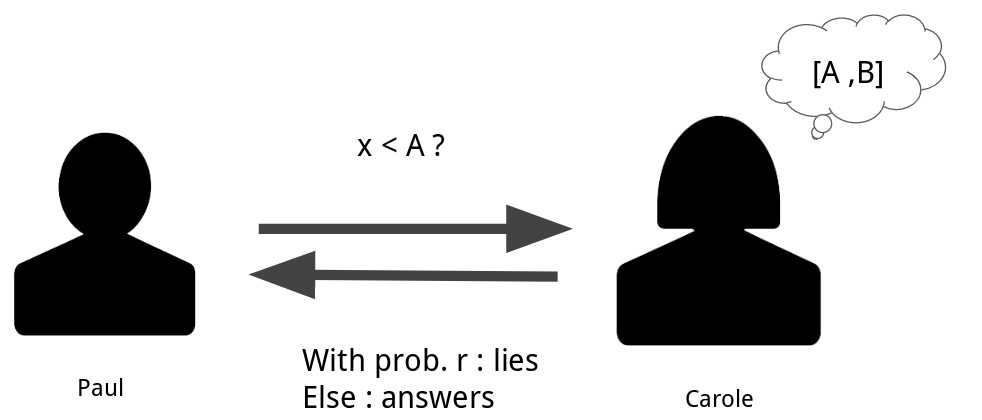
\includegraphics[width=0.8\textwidth]{figures/20q}
\end{center}

\begin{block}{[Dhagat, G{\'a}cs, Winkler '92]}
For $A = B$, Paul has a winning strategy for all $r < \frac{1}{3}$ asking $Q = \lceil \frac{8 \log N}{(1-3r)^2} \rceil =  \Theta(\log n)$ questions.
\end{block}

}

\frame{
\frametitle{Decision variant }

\btheme{Input:} integers ${k, \ell}$, a constant ${\eps > 0}$, strings ${S_1, S_2}$ of length ${n}$

\btheme{Output:} 

\begin{enumerate}
\item YES if ${\ell \le \mathrm{LCS_k}}$;
\item YES or NO if ${\mathrm{LCS_k} < \ell \le \mathrm{LCS_{(1+\eps)k}}}$; 
\item NO if ${\mathrm{LCS_{(1+\eps)k}} < \ell}$.
\end{enumerate}

The answer must be correct with probability at least $3/4$.

\pause
\par\noindent\ntheme{\rule{\textwidth}{1pt}}

\ntheme{Longest Common Substring with approx. $k$ mismatches:}

\medskip
\begin{itemize}
\item $A = \mathrm{LCS_k}$ and $B = \mathrm{LCS_{(1+\eps)k}}$.\\
\item An algorithm for the decision variant plays the role of Carole. \\
\item With ${\lceil \frac{8 \log n}{(1-3r)^2} \rceil}$ questions, Paul will find $x \in [\mathrm{LCS_k}, \mathrm{LCS_{(1+\eps)k}}]$ for some $1/4 < r < 1/3$.
\end{itemize}

}


\frame{
\frametitle{Locality-Sensitive Hashing}
Nearest Neighbour search, data clustering...\\
In string processing: Andoni and Indyk for a space-efficient randomized index for approximate pattern matching.
\pause
\begin{enumerate}
\item Projections:
\vspace{-0.5cm}
$$h(S)=S[a_{p_1}] S[a_{p_2}] \cdots S[a_{p_m}]$$
And Collisions-Sets (Karp-Rabin fingerprints).
$$\Collisions^{\Hashes}_{\ell} = \{(S_1,S_2, h) :\varphi(h(S_1 0^{n-\ell})) = \varphi(h(S_2 0^{n-\ell})) \}$$
\pause
\item Dimension reduction.
\vspace{0.1cm}
With probability at least $1- n^{-\beta}$, for all $u,v \in P$:\\
\begin{enumerate}[1)]
\item if $\norm{\sk_\alpha(u)-\sk_\alpha(v)}^2 \le (1+\alpha) \cdot k$, then $\HD(u,v) \le (1+\alpha) \cdot k$;
\item if $\norm{\sk_\alpha(u)-\sk_\alpha(v)}^2 > (1+\alpha) \cdot k$, then $\HD(u,v) \ge k$.
\end{enumerate}
\end{enumerate}
}



\frame{
\frametitle{Algorithm}

\begin{algorithm}[H]
\small
%\caption{LCS with approx. $k$ mismatches, decision variant}
\begin{algorithmic}[1]
\State Choose a set $\ntheme{\Hashes}$ of ${\Theta(n^{1/(1+\eps)})}$ functions from ${\Projections^m}$ u.a.r.
\State $\ntheme{\Collisions^{\Hashes}_{l} :=}$ set of all collisions of $l$-length substrings of $\ntheme{S_1, S_2}$ under the hash functions in $\ntheme{\Hashes}$
\State Draw a collision $\ntheme{(X, Y) \in \Collisions^{\Hashes}_{\ell}}$ uniformly at random 
\If {$\ntheme{\Ham (X, Y) \le (1+\eps) \cdot k}$}
	\Return YES
\EndIf
\State Choose a subset $\ntheme{\Collisions' \subseteq \Collisions^{\Hashes}_{l}}$ of size $\ntheme{\min\{\Collisions^{\Hashes}_{\ell}, 4nL\}}$
\For {$\ntheme{(X, Y) \in \Collisions'}$} 
	\If {$\ntheme{\Ham(S_1, S_2) \le k}$} 
		\Return YES
	\EndIf
\EndFor
\State \Return NO
\end{algorithmic}
\end{algorithm}

\pause
\ntheme{Running time $\Oh(n^{1+1/(1+\eps)} \log n)$:}
\begin{enumerate}
\item Compute the hash values and $\Collisions'$: $\Oh(n^{1+1/(1+\eps)} \log n)$ time (FFT)

\item Pick a random collision: $\Oh(n^{1+1/(1+\eps)})$ time (reservoir sampling)

\item Test in line 5: $\Oh(n^{1+1/(1+\eps)} \log^2 n)$ time (dimension reduction)

\item Test in line 7: $\Oh(n)$ time (character-by-character)
\end{enumerate}
}

\frame{
\frametitle{Experiments}

None of the previous solutions have been implemented. 

The only algorithm that seemed to be practical enough is the dynamic programming one \ntheme{[Flouri et al.'15]}

\pause
\bigskip

We compared our algorithm with the dynamic programming one
\begin{itemize}
 \item On random strings;
 \item On strings extracted from E. coli.
\end{itemize}

\medskip

Lengths from $5000$ to $60000$, $k = 10, 25, 50$
}

\frame{
\frametitle{Adjustments to the theory}
Implemented in C++ available on github.
\begin{enumerate}

\item Sketching for the Hamming distance via dimension reduction: replaced by a naive comparison character by character, Bit parallelism.
\pause

\item Computation of the collisions: A naive implementation, FFT and NTT.
\pause

\item The twenty question game: the twenty question game, binary search.
\pause

\item The number of hash functions $L$: $L = n^{1/(1+\eps)}$, $L = n^{1/(1+\eps)}/\log(n)$.

\end{enumerate}

}

\frame{
\frametitle{Running time}


\begin{figure}[ht!]
\centering
    \begin{subfigure}{.5\textwidth}
        \centering
        \captionsetup{justification=centering}
        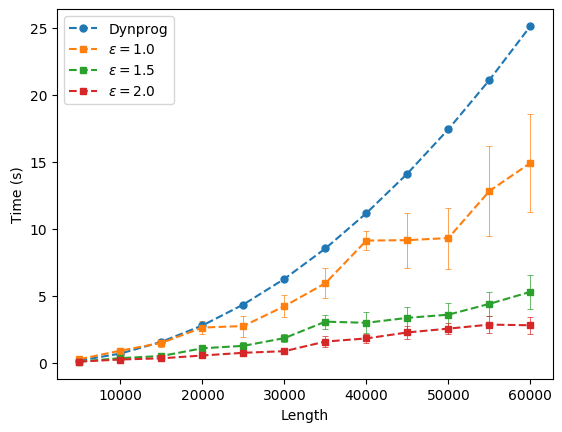
\includegraphics[scale=0.4]{figures/random_25.png}
        \caption{Random, $k = 25$}
    \end{subfigure}%
    \begin{subfigure}{0.5\textwidth}
        \centering
        \captionsetup{justification=centering}
        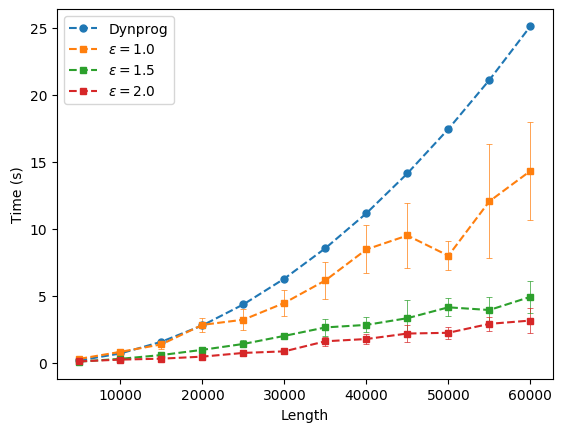
\includegraphics[scale=0.4]{figures/e_coli_25.png}
        \caption{E. coli, $k = 25$}
    \end{subfigure}     

\end{figure}


\bigskip

\begin{itemize}
\item For each length, we performed $10$ independent experiments
\item Big standard deviation for $\eps = 1$, negligible for $\eps = 1.5$ and $\eps = 2.0$
\item Gain up to a factor of 10 on strings of length $60000$
\end{itemize}
}



\frame{
\frametitle{Distortion and accuracy}

\begin{columns}
\column{0.5\textwidth}    
{\small
We estimate distortion by computing two values:

$r_{\min}(\eps, k) = \min_{S_1,S_2}(\mathrm{LCS_{\tilde{k}}}(S_1,S_2)/\mathrm{LCS_k}(S_1,S_2))$\\
$r_{\max}(\eps, k) = \max_{S_1,S_2}(\mathrm{LCS_{\tilde{k}}}(S_1,S_2)/\mathrm{LCS_k}(S_1,S_2))$

Furthermore, we can only err by returning a string shorter than $\mathrm{LCS_k}$.
}

\column{0.6\textwidth}

\newcolumntype{?}{!{\vrule width 1pt}}
\newcommand{\err}{\textcolor{red}{\mathrm{err}}}
\begin{center}
\begin{table}
\begin{tabular}{|l?l|l|l|l|l|l|}
\hline
 & \multicolumn{6}{c|}{\ntheme{Random}}\\ 
\hline
 & \multicolumn{2}{c|}{$\eps = 1.0$} & \multicolumn{2}{|c|}{$\eps = 1.5$} & \multicolumn{2}{|c|}{$\eps = 2.0$}\\ 
\hline

\multirow{ 2}{*}{$k = 10$} & 0.92 & 1.50 & 1.00 & 1.53 & 1.13 & 1.87\\ 
\cline{2-7}
& \multicolumn{2}{c|}{$\err = 7\%$}  & \multicolumn{2}{c|}{$\err = 0\%$}   & \multicolumn{2}{c|}{$\err = 0\%$}\\ 
\hline
\multirow{ 2}{*}{$k = 25$}  & 1.10 & 1.48 & 1.30 & 1.70 & 1.55 & 2.11\\ 
\cline{2-7}
& \multicolumn{2}{c|}{$\err = 0\%$}  & \multicolumn{2}{c|}{$\err = 0\%$}   & \multicolumn{2}{c|}{$\err = 0\%$}\\ 
\hline
\hline

& \multicolumn{6}{c|}{\ntheme{E. coli}} \\ 
\hline
& \multicolumn{2}{|c|}{$\eps = 1.0$} & \multicolumn{2}{c|}{$\eps = 1.5$} & \multicolumn{2}{c|}{$\eps = 2.0$} \\ 
\hline

\multirow{ 2}{*}{$k = 10$} & 0.86 & 1.41 & 0.91 & 1.47 & 0.95 & 1.71\\ 
\cline{2-7}
& \multicolumn{2}{|c|}{$\err = 34\%$}   & \multicolumn{2}{c|}{$\err = 13\%$}  & \multicolumn{2}{c|}{$\err = 8\%$}\\ 
\hline
\multirow{ 2}{*}{$k = 25$}  & 0.94  & 1.45 & 0.96 & 1.75 & 0.98 & 1.96\\ 
\cline{2-7}
& \multicolumn{2}{c|}{$\err = 7\%$}   & \multicolumn{2}{c|}{$\err = 5\%$}  & \multicolumn{2}{c|}{$\err = 2\%$}\\ 
\hline

\end{tabular} 
\label{tb:eps}
\end{table}
\end{center}


\end{columns}

}

\section{Bonus DTW}

\begin{frame}
  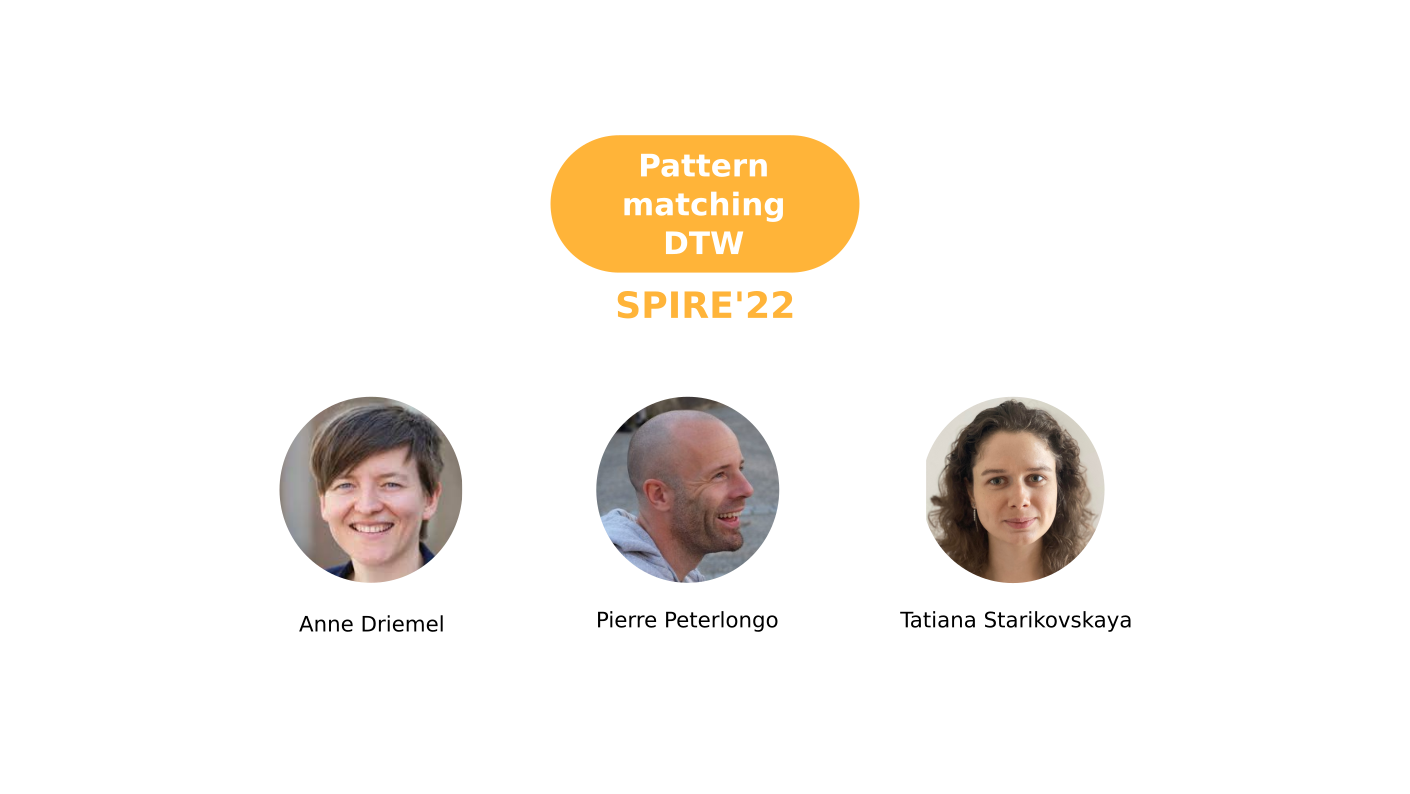
\includegraphics[width=\textwidth]{pictures/mindmap/dtw.png}
\end{frame}

\begin{frame}{Formal definition of $\dtw(X,Y)$ and dynamic programming}

  \begin{columns}
  \column{0.45\textwidth}
  \newcommand{\dtwgrid}[2]{% height width 
\foreach \i in {0,...,#1} {
	\foreach \j in {0,...,#2} {
		\filldraw[black] (\i , \j) circle (2pt);
		\ifthenelse{ \not \equal{#2}{\j}}{ 
			\draw[->] ($(\i , \j+0.9)$) -- ($(\i , \j+0.1)$);
		}{}
		\ifthenelse{ \not \equal{#1}{\i}}{
  			\draw[->] ($(\i +0.1 , \j)$) -- ($(\i +0.9 , \j)$);
		}{}
		\ifthenelse{\not\equal{#1}{\i} \and \not \equal{#2}{\j}}{%
  			\draw[->] ($(\i +0.1 , \j + 0.9)$) -- ($(\i +0.9, \j + 0.1)$);
  		}{}
	}
}
}

\newcommand{\dtwarrow}[2]{%
\draw[->,line width=0.3mm,red] #1 -- #2;
}

  \begin{figure}
      \beamermathcolor{black}
      \centering
      \begin{tikzpicture}[scale=0.8, every node/.style={scale=1.2}]
      \dtwgrid{5}{2}
  
      \foreach \i in {1,...,6} {
          \node at ($(\i-1, 2.8)$) {\tiny{$X[\i]$}};
      }
      \foreach \j in {1,...,3} {
          \node at ($(-1.2, 3 -\j )$) {\tiny{$Y[\j]$}};
      }
  
      \foreach \x[count=\i] in {C,A,A,A,G,G} {
          \node at ($(\i-1 , 2.3)$) {\textcolor{black}{\tiny{\x}}};
      }
      \foreach \y[count=\j] in {A,T,G} {
          \node at ($(-0.5, 3 -\j )$) {\textcolor{black}{\tiny{\y}}};
      }
  
  
      \only<2->{
          \dtwarrow{(0.1,2)}{(0.9,2)}
          \dtwarrow{(3.1,1.9)}{(3.9,1.1)}
          \dtwarrow{(1.1,2)}{(1.9,2)}
          \dtwarrow{(2.1,2)}{(2.9,2)}
          \dtwarrow{(4,0.9)}{(4,0.1)}
          \dtwarrow{(4.1,0)}{(4.9,0)}
          \node at (5,-0.3) {\bred{$\pi$}};
      }
  
      \end{tikzpicture}
  \end{figure}
  \column{0.45\textwidth}
  \centering
  \only<3>{
  $\text{cost}(\pi) = \sum_{(i,\ j)\in \pi} d(X[i],Y[j])$\\
  \vspace{0.5cm}
  $\dtw(X,Y) = \min_{\pi} \text{cost}(\pi)$\\
  \vspace{0.5cm}
  {\small s.t. $\pi$ goes from top left to bottom right.}}
  \end{columns}
  \pause %grid definition 
  \pause %draw the path
  \pause
  
  \bigskip
  
  
  \only<4|handout:0>{
  \begin{exampleblock}{Path correspondance to alignment}
  \center
  \begin{figure}
  %\missingfigure{Under construction...}
  \centering
  \begin{tikzpicture}[scale=0.7, every node/.style={scale=1}]
  \foreach \x[count=\i] in {C,A,A,A,G,G} {
      \node at ($(\i, 1)$) {\small{\x}};
  }
  \foreach \y[count=\j] in {A,T,G} {
      \node at ($(0.5+\j*1.5, 0)$) {\small{\y}};
  }
  % align A
  \fill[myblue!25] (2, 0.25) -- (2,0.75) -- (4,0.75) -- (2.1,0.25) -- cycle;
  % align G
  \fill[myblue!25] (5, 0.25) -- (5,0.75) -- (6,0.75) -- (5.1,0.25) -- cycle;
  %draw misalignment
  \draw[dashed,red] (1.75, 0.25) -- (1,0.75);
  \draw[dashed,red] (3.5, 0.25) -- (5,0.75);
  \end{tikzpicture}
  \end{figure}
  \vfill
  $\dtw($CAAAG$,$ATG$)=2$
  \end{exampleblock}}
  
  \only<5->{
  
  \btheme{Dynamic Programming solution}\\
  \smallskip
  $D$ a matrix of size $(M+1)(N+1)$ such that $D[i,j]=\dtw(X[1..i],Y[1..j])$\pause
  \bigskip
  
  \btheme{Initialization}~~~$D[0,0]= 0$ and for all $(i,j)$, $D[0,j]=D[i,0]=+\infty$.\\
  \pause
  \bigskip
  \btheme{Recurrence} ~~~ 
      $D[i,j] = \min\{$\beamermathcolor{black}
          $\underbrace{\mathcolor{black!30!blue}{D[i-1,j-1]}}_\text{top-left},
          \underbrace{\mathcolor{black!30!blue}{D[i-1,j]}}_\text{top},
          \underbrace{\mathcolor{black!30!blue}{D[i,j-1]}}_\text{left}$
      $\mathcolor{black!30!blue}{\}+ d(X[i], Y[j])}$.
  }
  
  \end{frame}
  

\begin{frame}{}

  \textbf{Our contributions:}\\
  For $T$ and $P$ two strings, $|T|=N$ and  $|P|=M$, $|\RLE(T)|=n$ and  $|\RLE(P)|=m$.
  Pattern matching under DTW distance:
  \begin{itemize}
  \item $\Oh(Nm+nM)$-time general algorithm which can for an integer distance, compute all values bellow $k$ in $\Oh(nmk)$-time. \pause
  \item Toy implementation available on github.\pause
  \item An $\Oh(L^{\eps})$-approximation, for any $0 < \eps < 1$, in  $\Oh(L^{1-\eps} \cdot mn \log^3 L)$-time with $L=\max(N,M)$.\pause
  \item (A $\Oh(n+m)$-time algorithm for $k=1$.)\pause
  \end{itemize}
  
  
  \textbf{Open questions:}
  \begin{itemize}
  \item Is a $\Oh(k(n+m))$-time algorithm possible? \pause
  \item Can those improvements benefit applications ?\pause
  \end{itemize}
  \end{frame}


\begin{frame}{Experiments: visualization on simulated data}
  Problem: How to design a protocol that isn't biased towards ED ?\\
  Model to illustrate the impact of homopolymers on ED.
  \begin{center}
    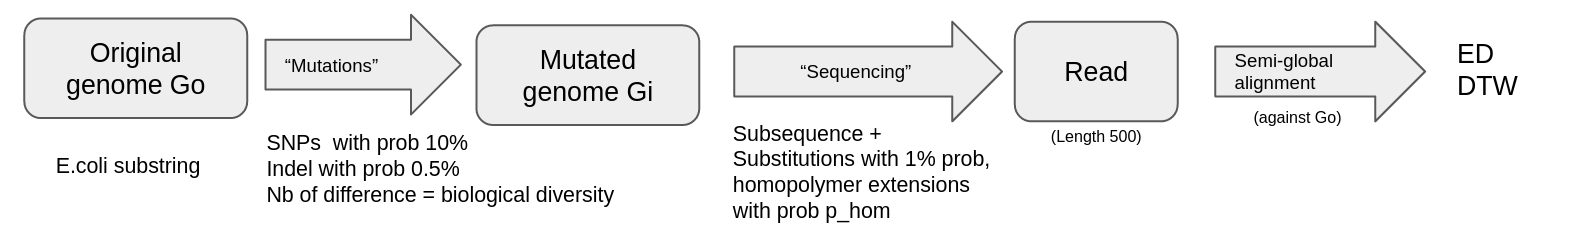
\includegraphics[scale=0.2]{figures/pipeline.png}
  \end{center}
  \vspace{-0.5cm}
  \begin{columns}
    \column{0.3\textwidth}
    
    We compare the values of the two distances as the probability of extending homopolymers increases.
    
    \column{0.5\textwidth}
    \begin{center}
      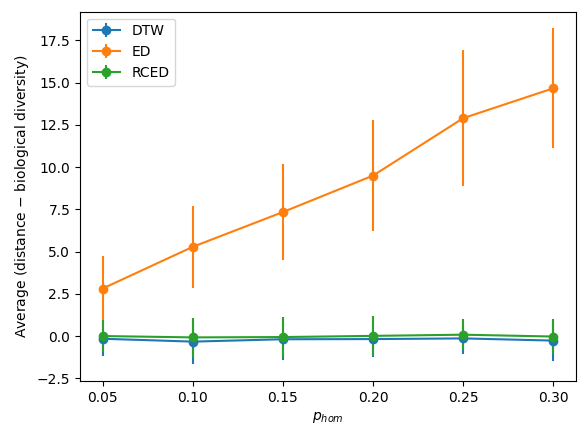
\includegraphics[scale=0.4]{figures/ecoli_10kb_N_100_fixed_ID_0.0005.png}
    \end{center}
  \end{columns}
\end{frame}


\begin{frame}{Comparison to the edit distance}
  \beamermathcolor{black}
  \[
  D[i,j] = {\min\{
  \underbrace{D[i-1,j-1]}_\text{top-left},
  \underbrace{D[i-1,j]}_\text{top},
  \underbrace{D[i,j-1]}_\text{left}
  \} \mathcolor{red}{+ d(X[i], Y[j])}
  }
      \]
  
  \[
  ED[i,j] = {\min\{
  \underbrace{ED[i-1,j-1]}_\text{top-left} \mathcolor{red}{+ d(X[i], Y[j])},
  \underbrace{ED[i-1,j]}_\text{top} \mathcolor{red}{+1},
  \underbrace{ED[i,j-1]}_\text{left} \mathcolor{red}{+1}
  \}
  }
      \]
  
  \pause
  
  \only<2-3|handout:0>{
  \begin{exampleblock}{DTW vs ED}
  $\ed(AAAA\mathcolor{myblue}{T}G,AA\mathcolor{myblue}{T}C)=3$ whereas $\dtw(AAAA\mathcolor{myblue}{T}G,AA\mathcolor{myblue}{T}C)=1$.\\
  $\dtw(AAAA\mathcolor{myblue}{T}G,AA\mathcolor{myblue}{T}CCC)=3$
  \end{exampleblock} 
  
  \only<3>{$\Rightarrow$ Compresses runs of matching letters!}
  }

  \only<4>{
    \begin{center}
      
\begin{center}
\footnotesize
\resizebox{0.8\textwidth}{!}{
\begin{tabular}{|cc||cc|cccc|c|cc|c|cccc|cc|c|c|c|c|c|}
\hline
 &   & G & G & T & T & T & T & C & T & T & A & T & T & T & T & G & G & T & G & A & T & A \\
 & 0 & 0 & 0 & 0 & \textcolor{red}{0} & 0 & 0 & 0 & 0 & 0 & 0 & 0 & 0 & 0 & 0 & 0 & 0 & 0 & 0 & 0 & 0 & 0 \\
\hline
A  & $\infty$  & 1 & 1 & 1 & 1 & \textcolor{red}{1} & 1 & 1 & 1 & 1 &{ 0 } & 1 & 1 & 1 & 1 & 1 & 1 & 1 & 1 &{ 0 } & 1 &{ 0 }\\
A  & $\infty$  & 2 & 2 & 2 & 2 & 2 & \textcolor{red}{2} & 2 & 2 & 2 &{ 0 } & 1 & 2 & 2 & 2 & 2 & 2 & 2 & 2 &{ 0 } & 1 &{ 0 }\\
\hline
T  & $\infty$  & 3 & 3 &{ 2 } &{ 2 } &{ 2 } &{ 2 } & \textcolor{red}{3} &{{ 2 }} &{{ 2 }} & 1 &{ 0 } &{ 0 } &{ 0 } &{ 0 } & 1 & 2 &{ 2 } & 3 & 1 &{ 0 } & 1\\
T  & $\infty$  & 4 & 4 &{ 2 } &{ 2 } &{ 2 } &{ 2 } & 3 & \textcolor{red}{{ 2 }} &{{ 2 }} & 2 &{ 0 } &{ 0 } &{ 0 } &{ 0 } & 1 & 2 &{ 2 } & 3 & 2 &{ 0 } & 1\\
\hline
A  & $\infty$  & 5 & 5 & 3 & 3 & 3 & 3 & 3 & 3 & \textcolor{red}{3} &{{ 2 }} & 1 & 1 & 1 & 1 & 1 & 2 & 3 & 3 &{ 2 } & 1 &{ 0 }\\
\hline
T  & $\infty$  & 6 & 6 &{ 3 } &{ 3 } &{ 3 } &{ 3 } & 4 &{ 3 } &{ 3 } & \textcolor{red}{3} &{{ 1 }} &{{ 1 }} &{{ 1 }} &{{ 1 }} & 2 & 2 &{ 2 } & 3 & 3 &{ 1 } & 1\\
\hline

\end{tabular} }
\end{center}



\pause
    \end{center}
    \small{Unlike for the edit distance, \textcolor{red}{diagonals can be non-monotone}.}
  }
      
  \end{frame}

\section{XBWT indexing of aligned readsets}
\begin{frame}
  \centering
  {\Large XBWT indexing of aligned readsets}
    
  \medskip
  {\large WABI'21}
  \bigskip

  
\includegraphics{pictures/mindmap/xbwt.png}

  \bigskip
  Travis Gagie, Giovanni Manzini
\end{frame}

%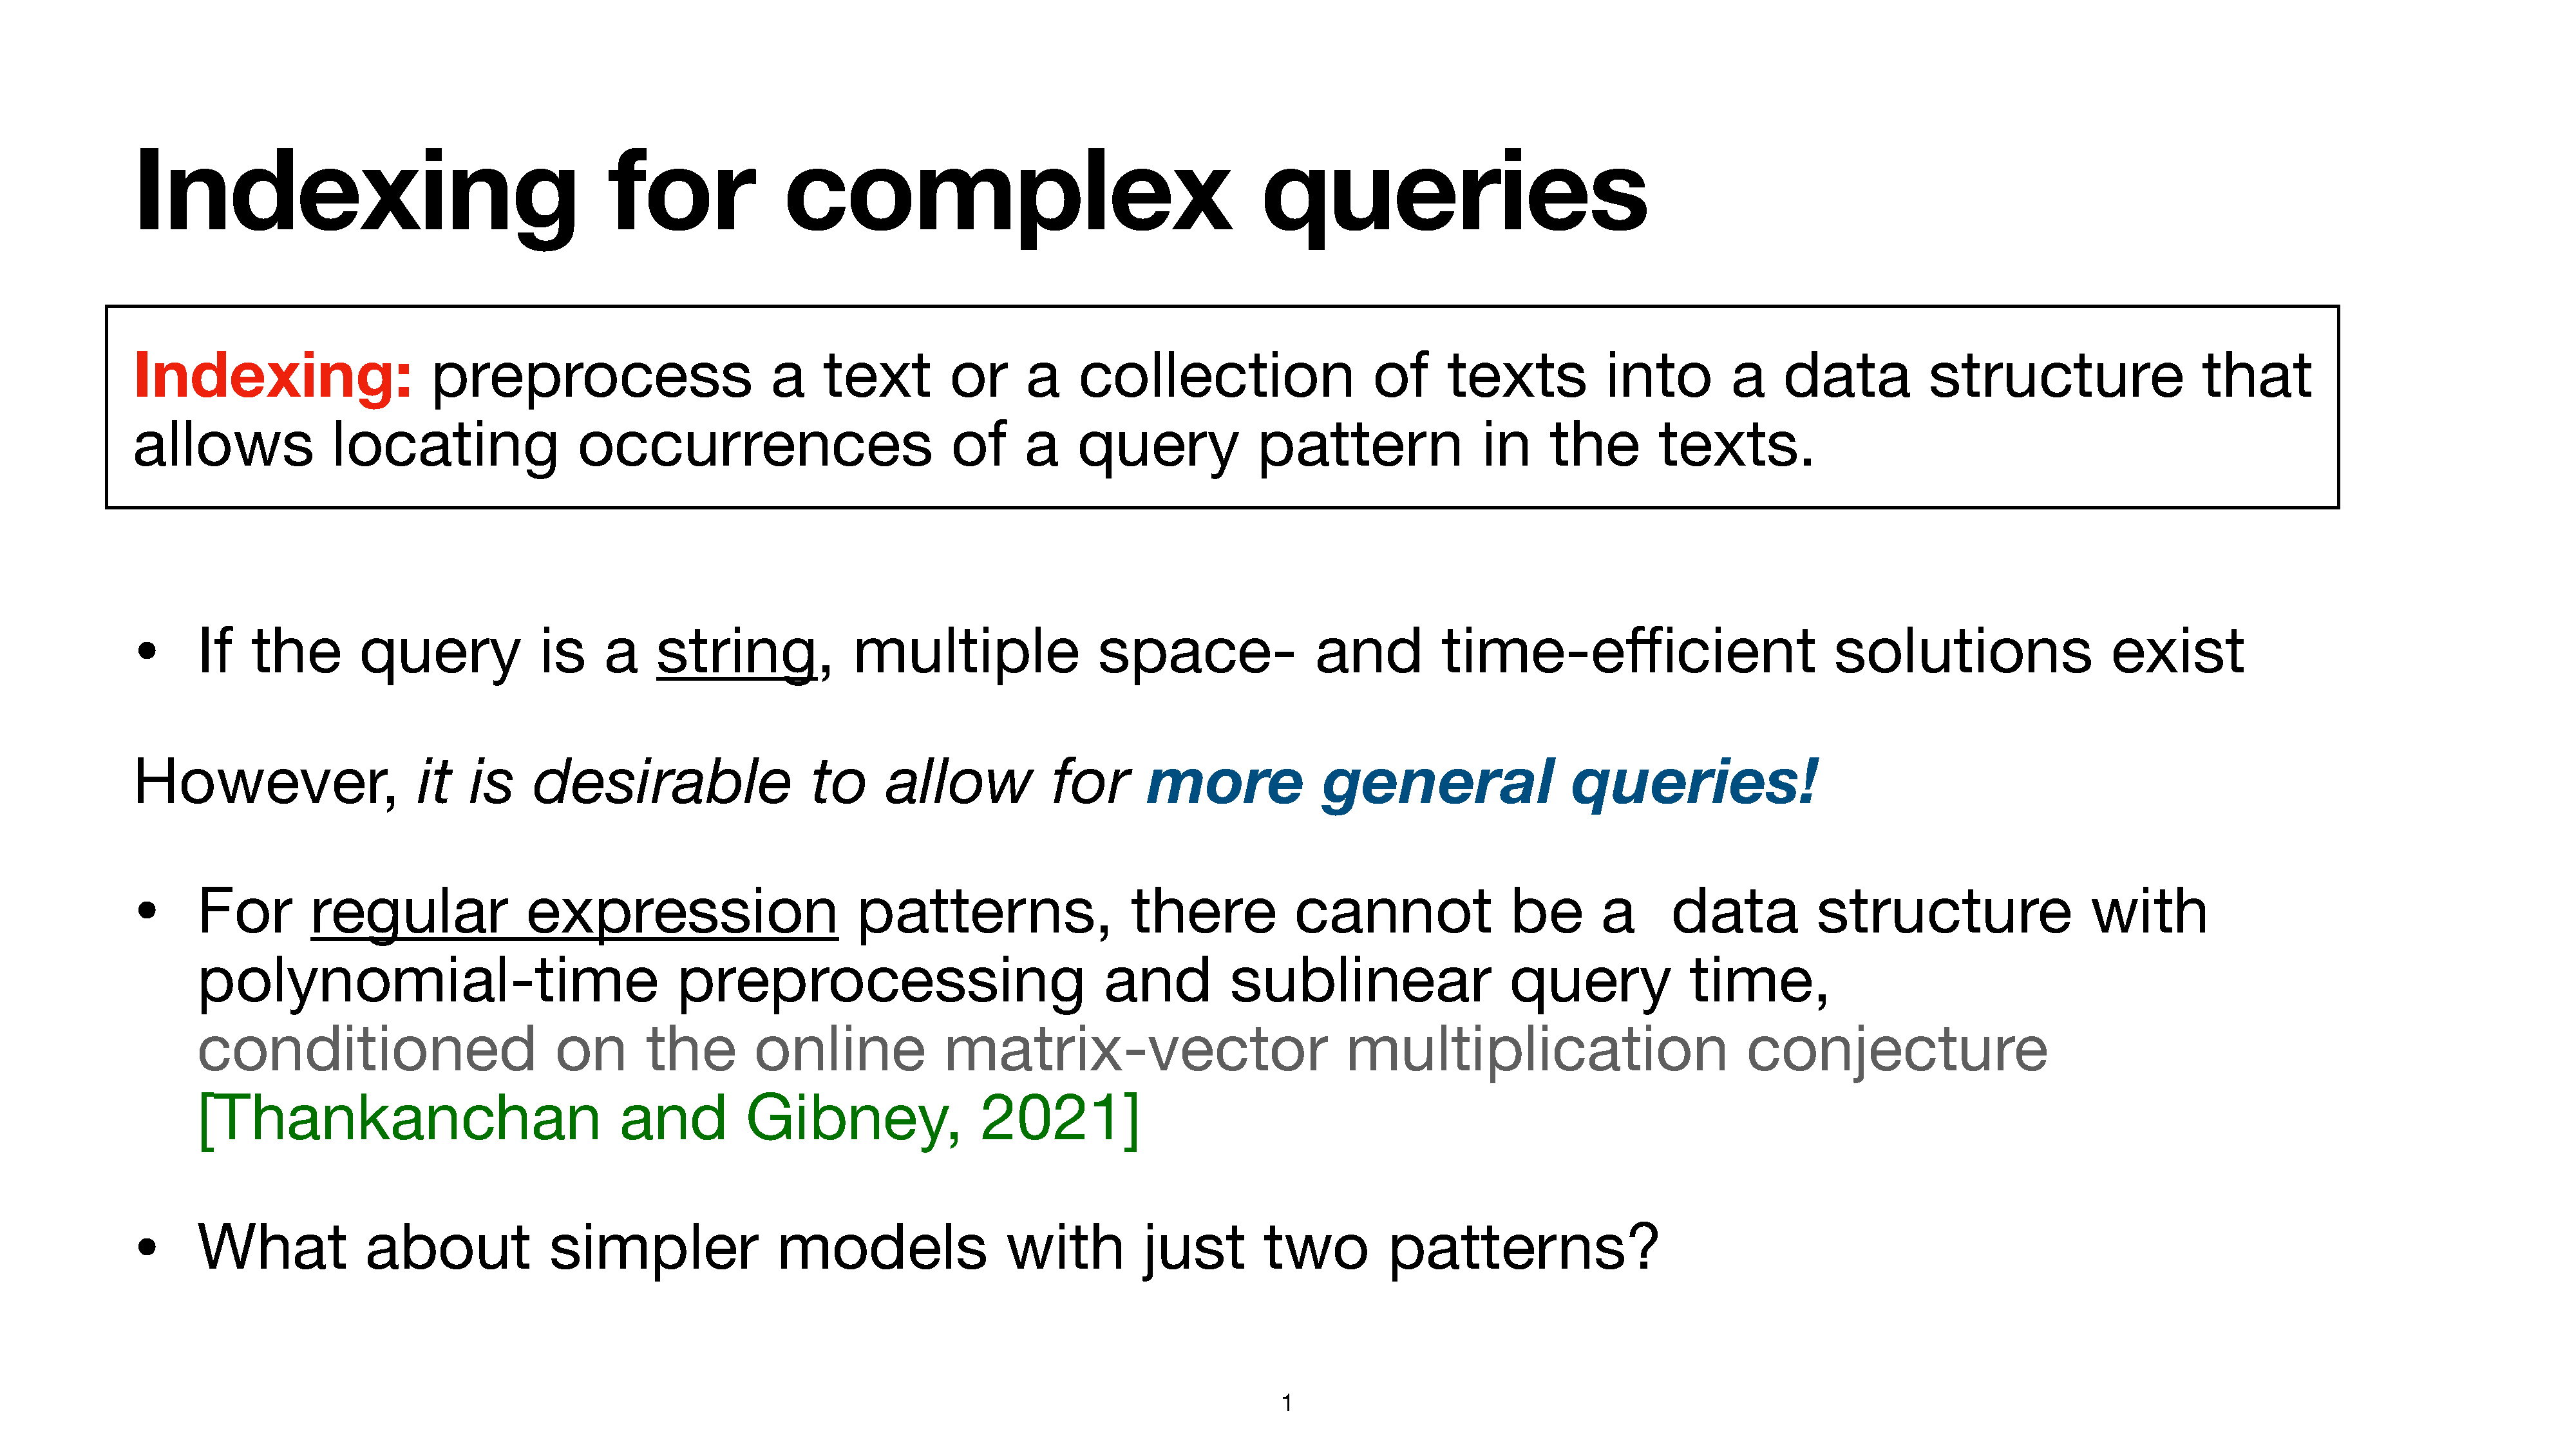
\includepdf[pages={-}]{pdf/2_index_gapped.pdf}

\backupend

